\chapter{Descripcion}\label{chapter04}
\section{Arquitectura de la solución}\label{sec:arquitectura-solucion}
En esta sección se presenta la arquitectura de SmartStocker, detallando las tecnologías empleadas para su diseño técnico y funcional. La arquitectura funciona como marco conceptual que sustenta cada componente del sistema y especifica las interacciones y dependencias entre las distintas partes que lo componen.

\subsection{Diagrama de Arquitectura conceptual}\label{sec:arquitectura-conceptual}
En relación con la arquitectura de alto nivel de SmartStocker, se propone un modelo de tres capas que organiza la solución, asegurando una separación clara de responsabilidades y mejorando la escalabilidad. Esta estructura está diseñada para optimizar tanto la interacción con el usuario como el procesamiento y almacenamiento de los registros de venta y los resultados de inferencia generados por los modelos predictivos.

La primera capa —Capa de Presentación (Presentation Layer)— agrupa la interfaz y la experiencia de usuario. En ella se implementa el frontend de SmartStocker con Next.js y se despliega mediante AWS Amplify, aprovechando sus capacidades de hosting y CI/CD. Esta capa permite a los usuarios interactuar con la plataforma, gestionar sus productos e ingredientes, visualizar recomendaciones y alertas, y realizar operaciones de predicciones de venta de forma responsiva y orientada a la operativa diaria.

La Capa de Negocio (Business Layer) constituye el núcleo lógico de SmartStocker y se organiza en tres componentes principales. El primero es una API REST que actúa como puente entre la capa de presentación y los servicios backend; a través de ella se gestionan las sesiones y la autorización, se exponen los endpoints para solicitar predicciones y gestionar productos, ingredientes, y alertas, y se que incluye la lógica necesaria para atender las demandas de la interfaz de usuario de forma segura y consistente. El segundo es el pipeline de ETL, encargado de recibir los datos de ventas en tiempo real desde los sistemas externos, procesarlos, enriquecerlos, y dejarlos listos para ser usados por el modelo. Por último, el pipeline de ML será el encargado de realizar el entrenamiento del modelo, ya sea de forma periódica u on demand, y de dejarlo disponible para su uso en las operaciones de inferencia 

Por último, la Capa de Almacenamiento (Storage Layer) se organiza según los distintos casos de uso de la plataforma y está diseñada para optimizar rendimiento y costos. Los datos de la aplicación, tales como los ingredientes, productos, ventas realizadas,  y resultados de predicciones, se almacenan en DocumentDB, lo que facilita lecturas de baja latencia y flexibilidad en la estructura de los datos. Mientras tanto, los datos orientados al entrenamiento del modelo, tales como los datasets históricos, los artefactos de entrenamiento y los modelos exportados se almacenan en Amazon S3, aprovechando su durabilidad y su bajo costo.

\begin{figure}[htbp]
    \centering
    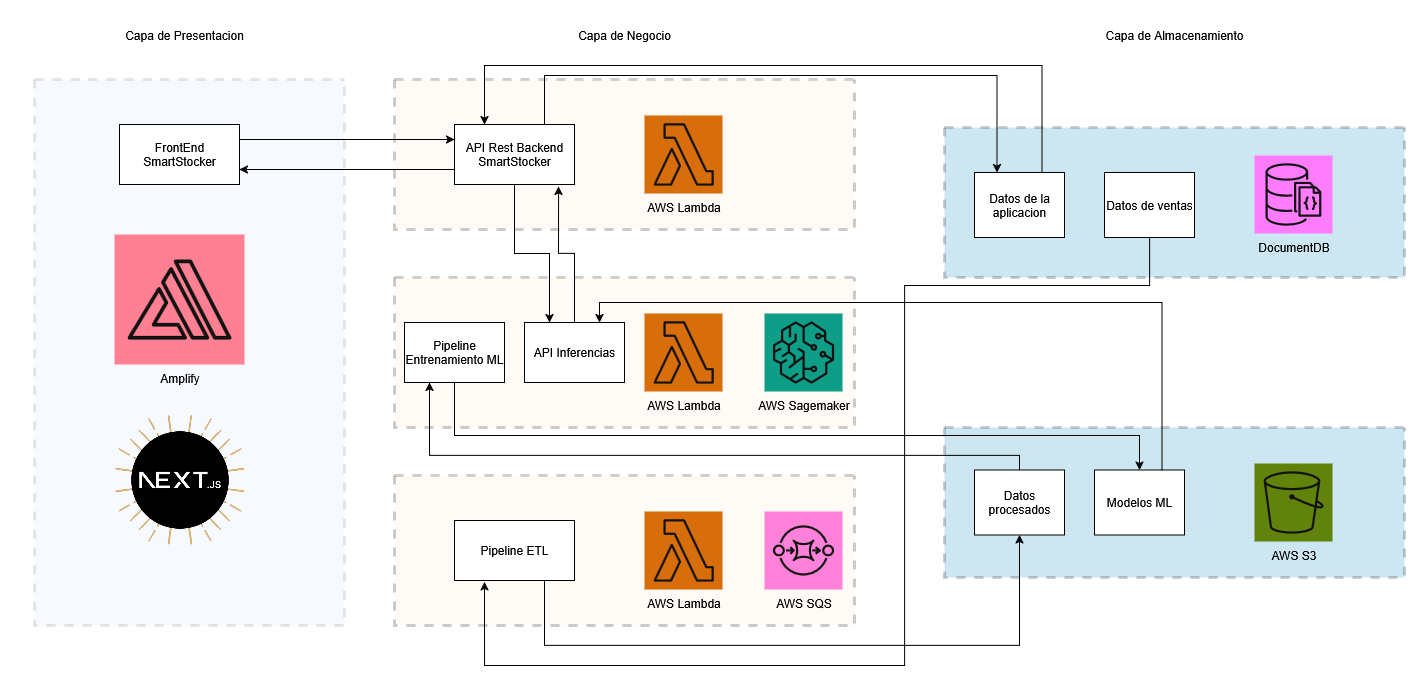
\includegraphics[width=0.7\textwidth]{images/arquitectura_capas.png}
    \caption{Arquitectura conceptual de SmartStocker}
    \label{fig:arquitectura-conceptual}
\end{figure}

\subsection{Diagrama de Despliegue}\label{sec:arquitectura-despliegue}
Se decidió usar Amazon Web Services (AWS) como solución de despliegue para nuestra solución, debido a la flexibilidad y amplitud de herramientas ofrecidas necesarias para implementar la arquitectura de SmartStocker.

Analizando la capa de presentación, esta se encuentra desarrollado con Next.js, y desplegado a través de AWS Amplify. Se eligió este servicio puesto que simplifica enormemente la gestión de la aplicación, permitiendo, mediante una simple configuración inicial, encargarse de aspectos tales como el despliegue (permitiendo CI/CD integrado a GitHub), hasta del escalamiento en sí.

Para la capa de almacenamiento, se optaron por dos soluciones. Primero, DocumentDB como base de datos NoSQL, seleccionado debido a la naturaleza no estructurada de los datos a utilizar, y que nos brinda la posibilidad de modificar el schema con facilidad, además de ser una base serverless escalable. Y segundo, S3, para contener la información en formato csv requerida para los entrenamientos del modelo, y para almacenar los archivos correspondientes al modelo entrenado en si.

Para la capa de negocio, se decidió implementar las distintas APIs requeridas mediante AWS Lambda, dado que su enfoque serverless permite abstraernos de la gestión de la infraestructura, acelerando el desarrollo y la puesta en producción, escalando cuando la demanda lo requiera, y reduciendo los costos fijos.

Esto también aplica para el pipeline de ETL, donde también se utiliza AWS Simple Queue Service (SQS) para desacoplar el procesamiento de las ventas, a fin de lograr velocidades de respuesta rápida ante los sistemas externos que enviaran las mismas, mientras que el procesamiento y enriquecimiento de las ventas se realiza en otra Lambda.

Por último, se decidió usar AWS Sagemaker en el pipeline de ML, puesto que simplifica enormemente el entrenamiento del modelo, requiriendo suministrarle solamente el dataset a utilizar, y permite disponibilizar el modelo para ser usado para predicciones mediante endpoints, lo que brinda una consulta rápida y de facil implementacion.

\begin{figure}[htbp]
    \centering
    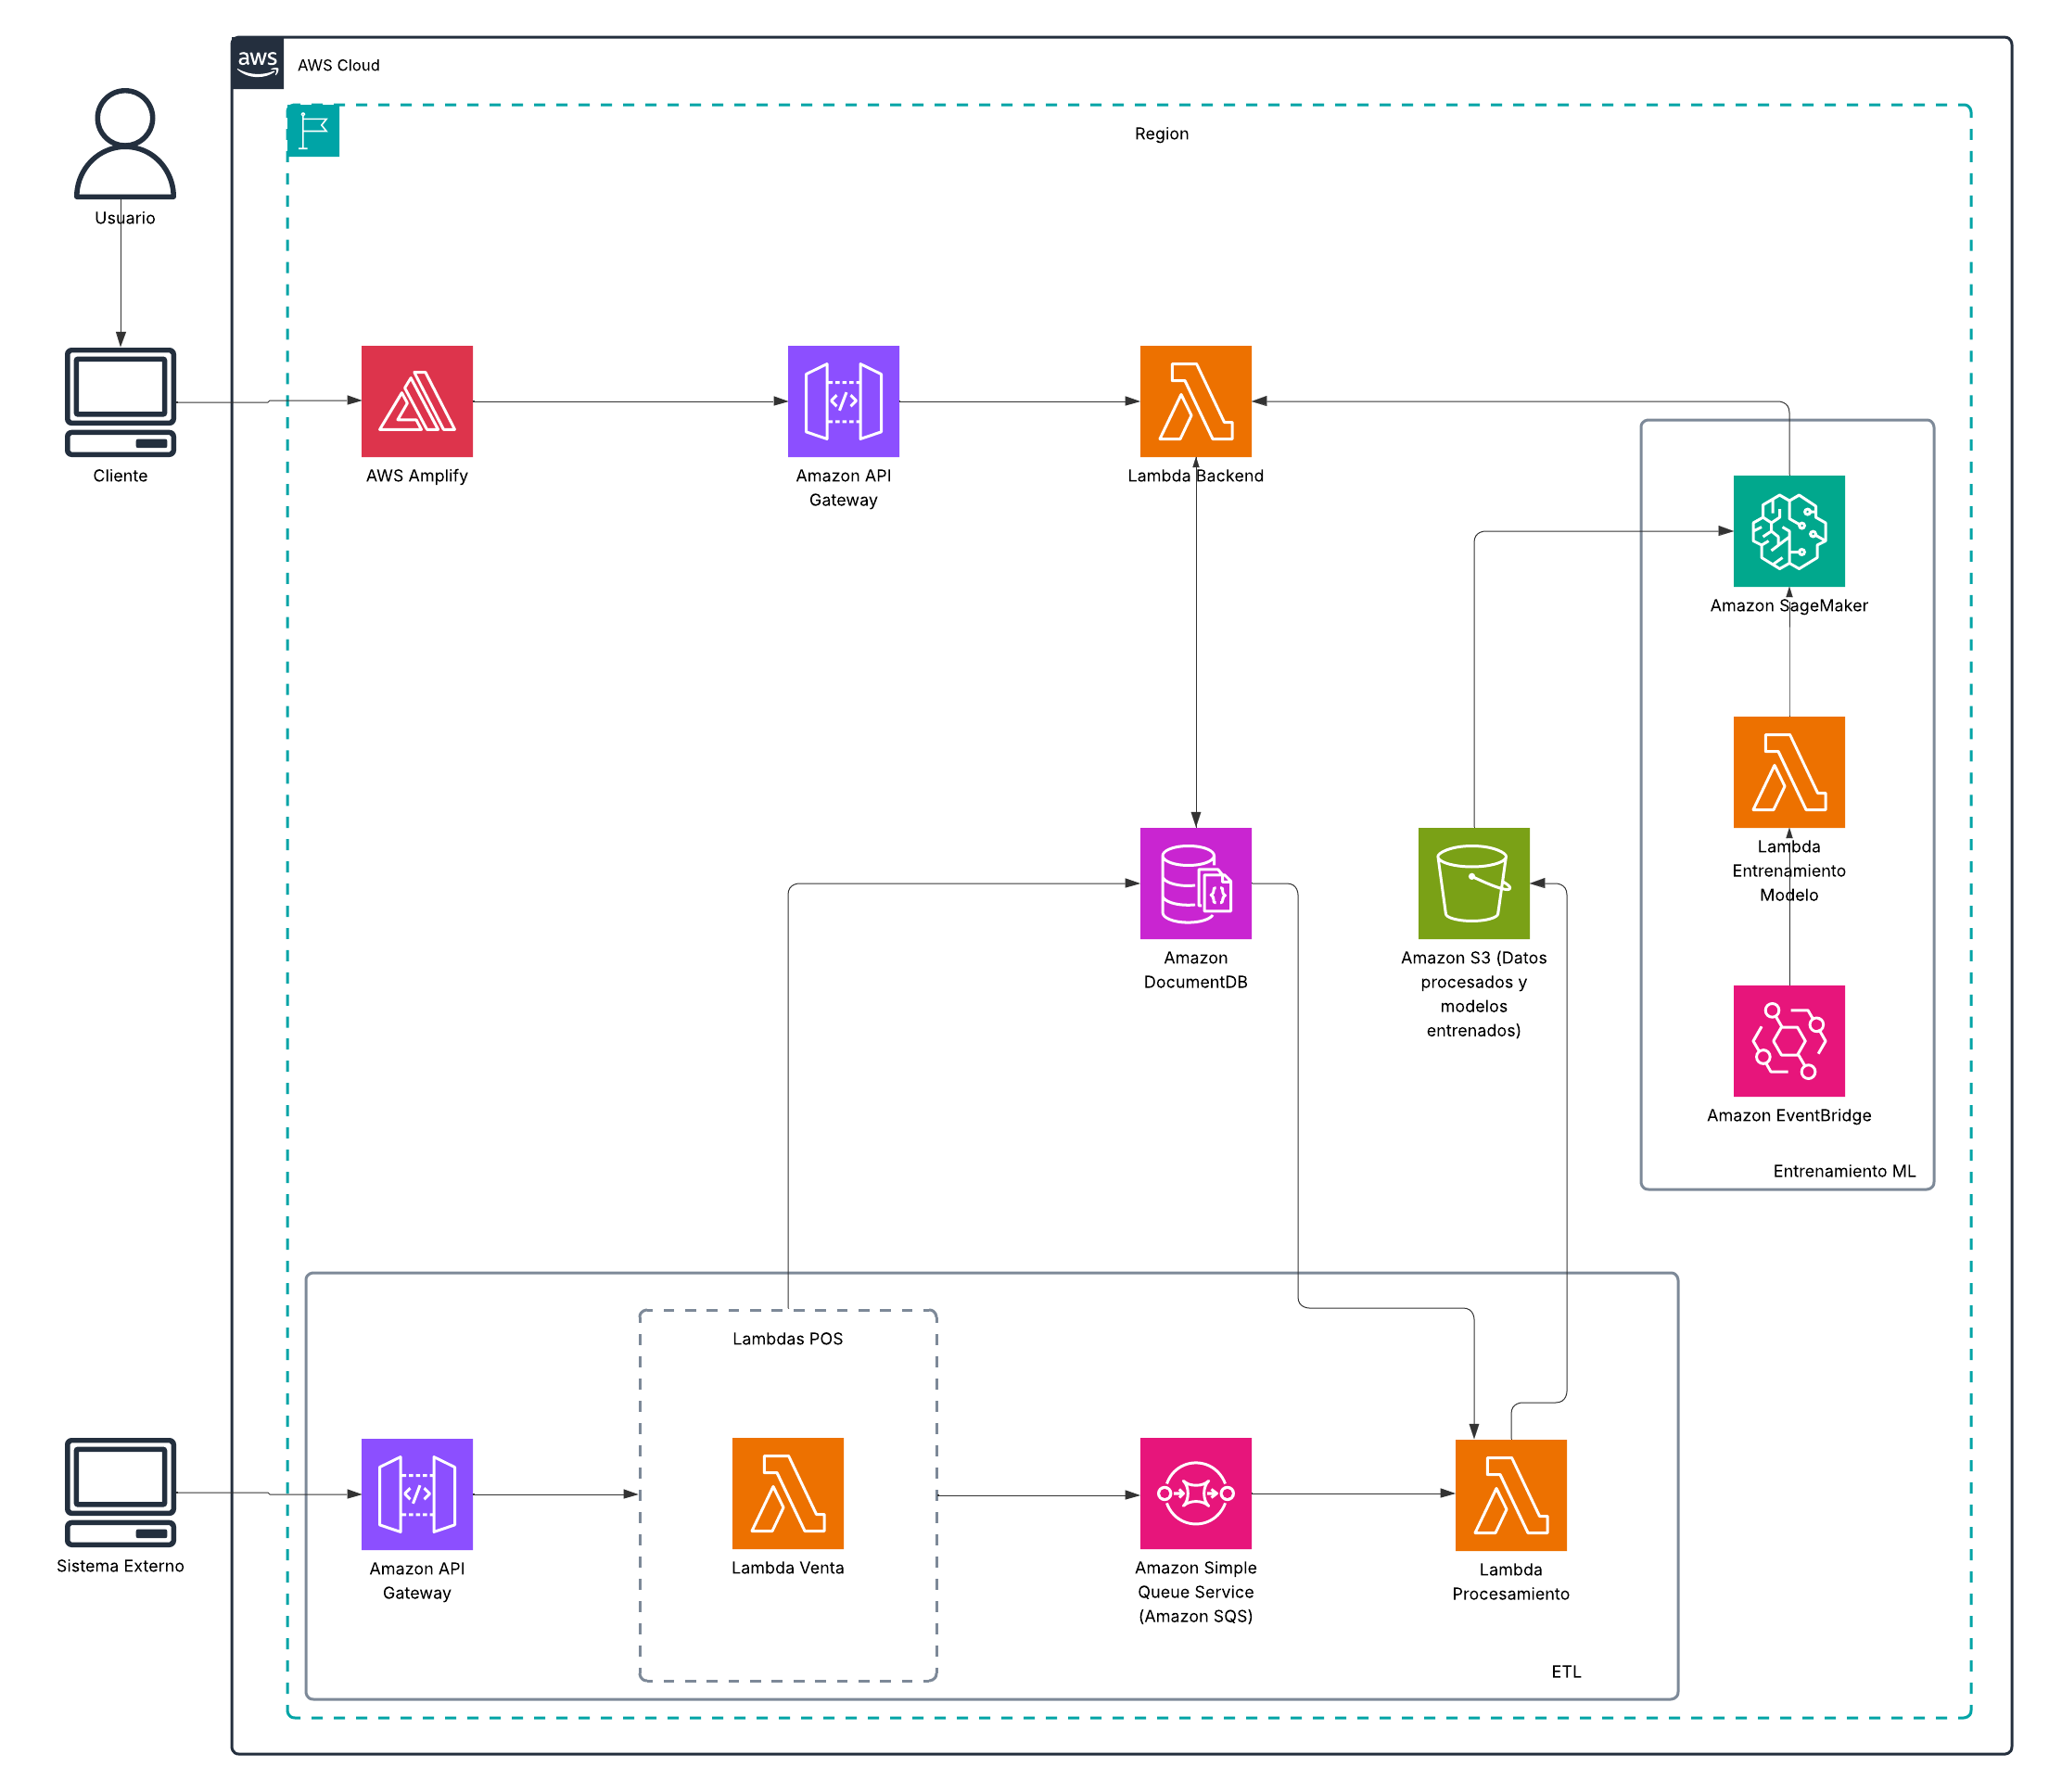
\includegraphics[width=0.7\textwidth]{images/arquitectura_despliegue.png}
    \caption{Arquitectura de Despliegue y Procesos de SmartStocker}
    \label{fig:arquitectura-despliegue}
\end{figure}

\subsection{Diagrama de Base de datos}\label{sec:arquitectura-base-datos}

Para el diseño de la base de datos, se opto por utilizar DocumentDB, una de las alternativas NoSQL brindadas por AWS, debido a la flexibilidad y capacidades de escalado automatico que esta nos provee, siendo la flexibilidad del schema algo critico dada la necesidad de agregar campos adicionales conforme el proceso de ETL o entrenamiento del modelo de ML lo requieran.

El diseño de la base de datos se organiza alrededor de cinco entidades principales: Usuario, ItemMenu, Ingrediente, Predicción y Venta. La entidad Usuario representa a un negocio dentro de la plataforma. A su vez, la entidad Ingrediente almacena los insumos (nombre, unidad de medida, cantidad en stock y cantidad mínima) y su propietario (userId), mientras que ItemMenu registra los productos ofrecidos (código, nombre, estado activo) y contiene la lista de ingredientes necesarios para cada receta. Esa relación N:M entre ItemMenu e Ingrediente se materializa en la tabla/intersección (el subdocumento de ingredientes) que guarda, por cada par producto-ingrediente, la cantidad\_requerida. La entidad Predicción registra las predicciones de demanda vinculadas a un producto\_id (ItemMenu) con fecha\_prediccion, turno, cantidad\_predicha y el userId que la generó; y la entidad Venta recoge las transacciones reales (número de venta, ítem, producto, cantidad, precio unitario, subtotal, fecha, turno, plataforma, método de pago y estado) asociadas también a un userId. Todos los documentos incluyen timestamps (fecha\_creacion / fecha\_actualizacion) para auditoría.

\begin{figure}[htbp]
    \centering
    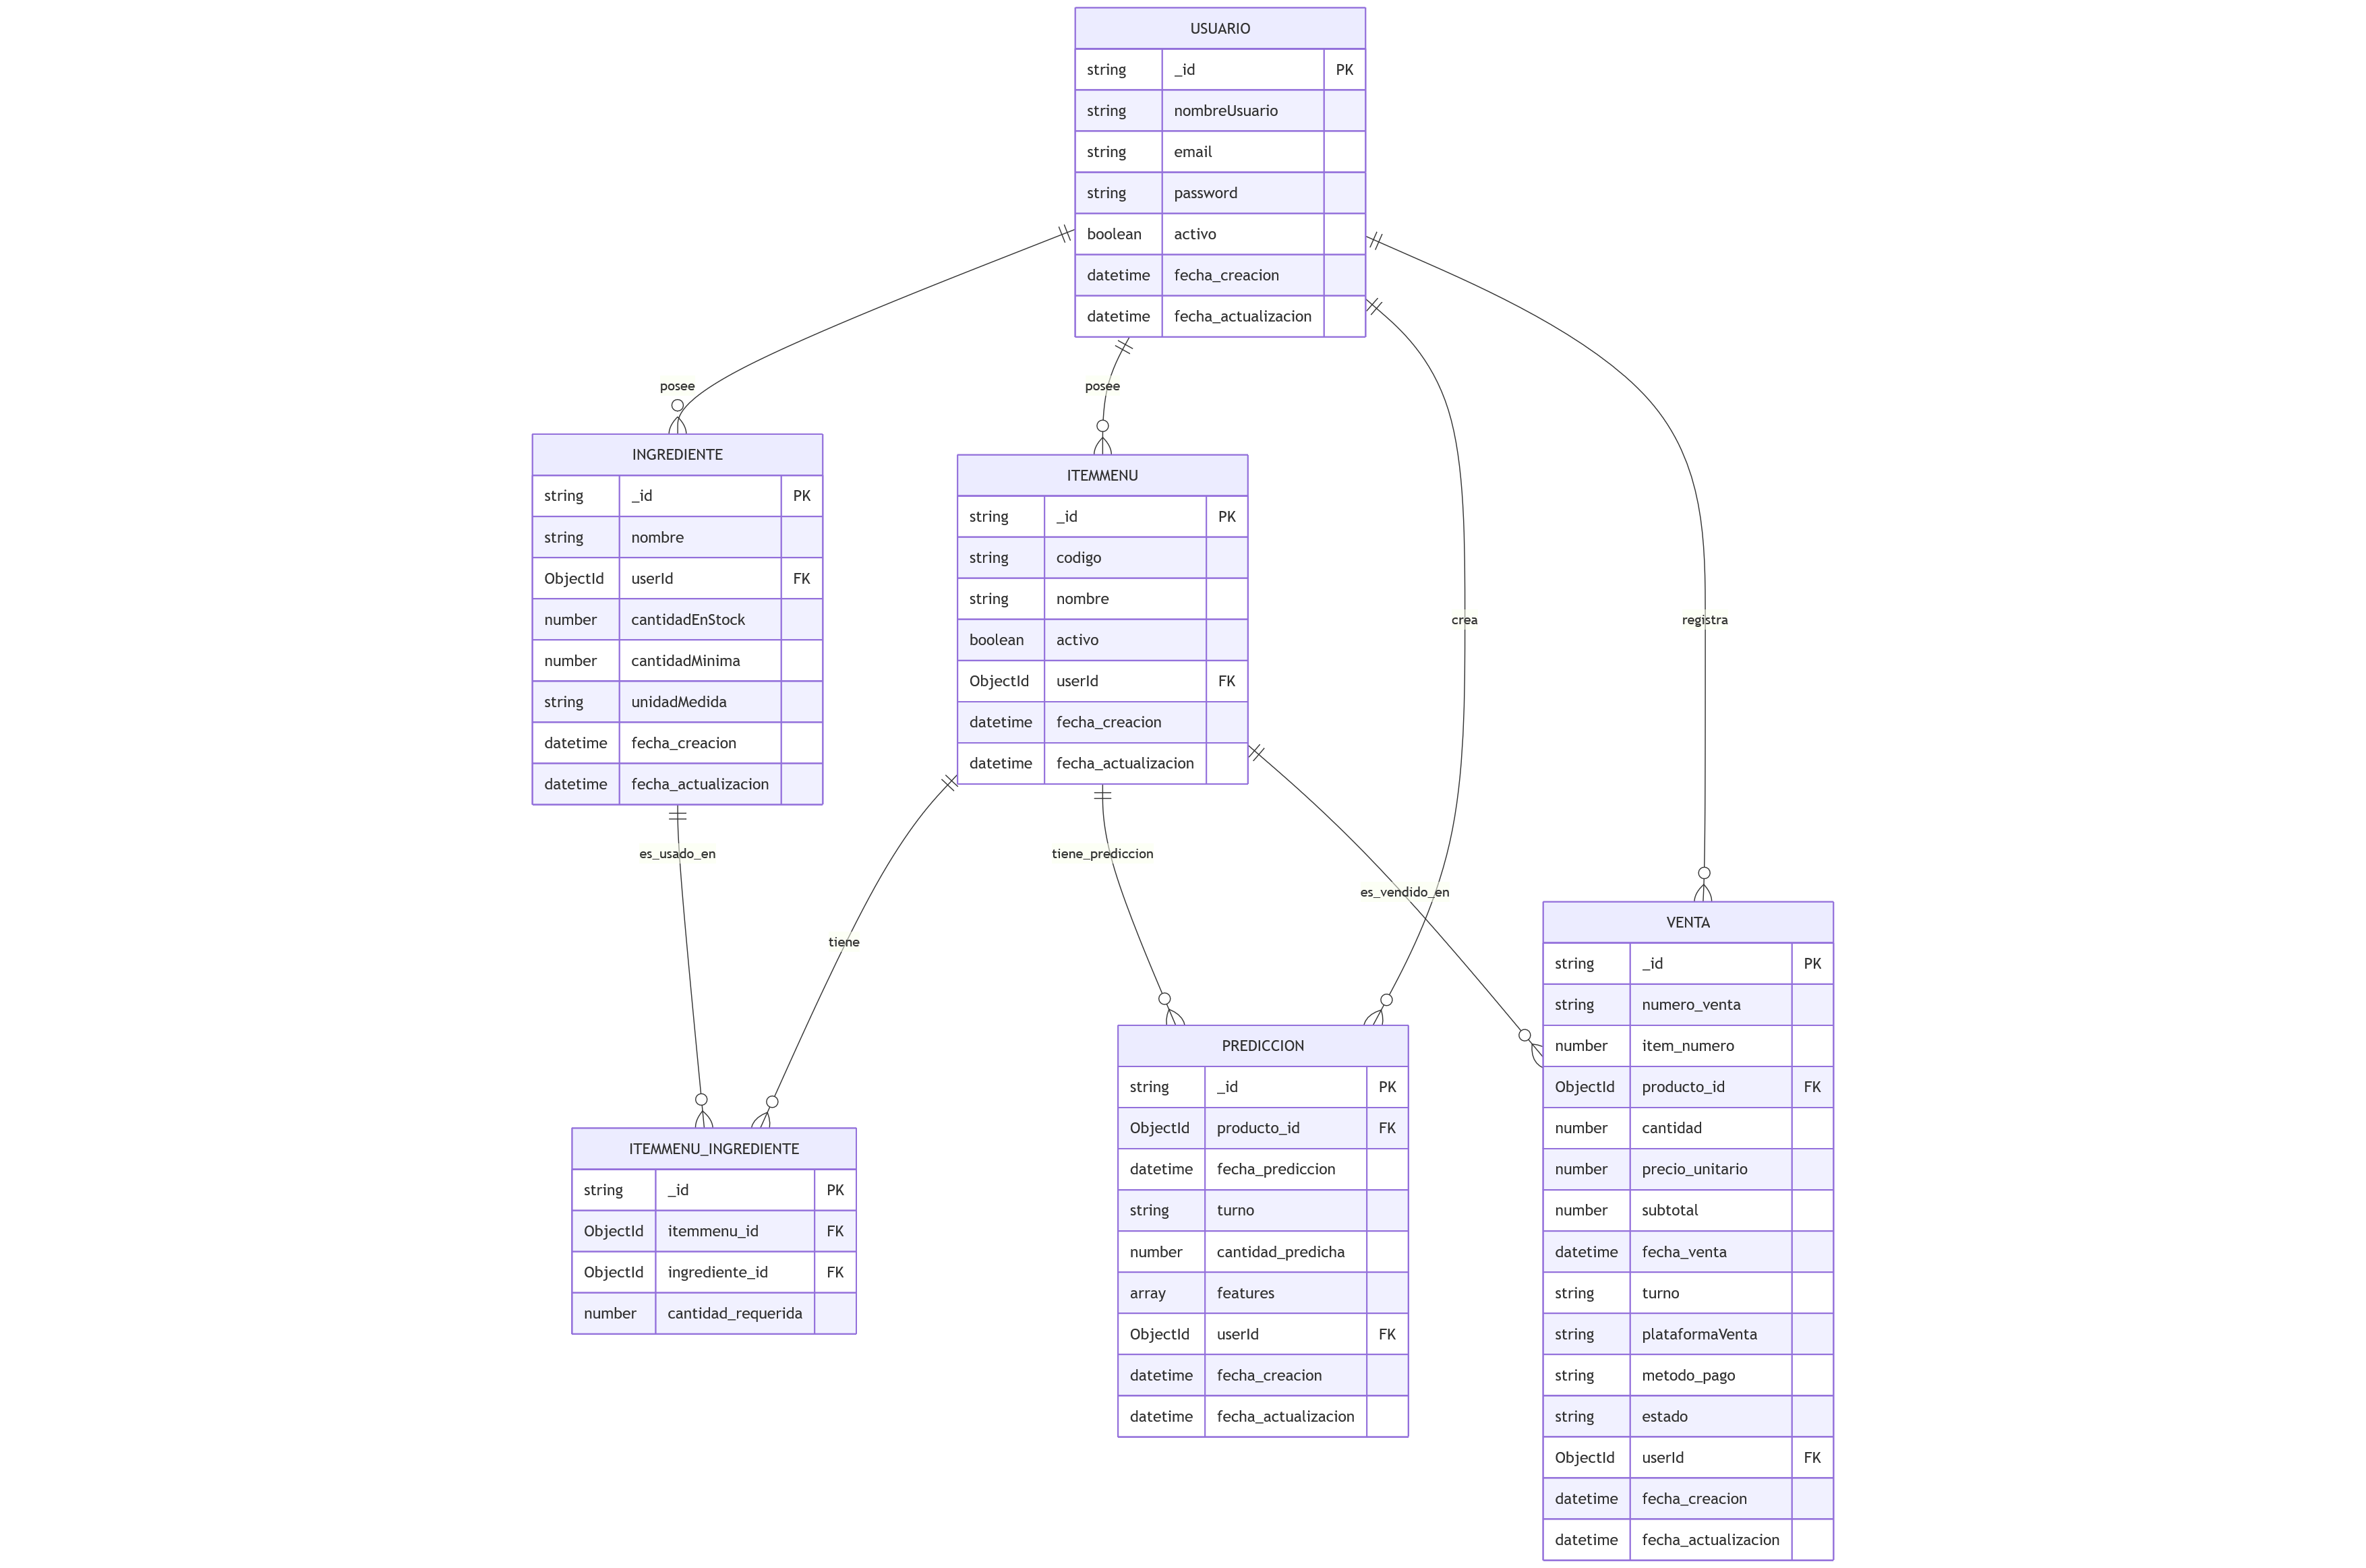
\includegraphics[width=0.7\textwidth]{images/arquitectura-base-datos.png}
    \caption{Arquitectura de Base de Datos de SmartStocker}
    \label{fig:arquitectura-base-datos}
\end{figure}

\subsection{Pipeline Machine Learning}\label{sec:pipeline-machine-learning}

El pipeline de entrenamiento del modelo de machine learning se encuentra implementado mediante el uso de AWS EventBridge, a fin de programar entrenamientos periódicos de forma semanal. El EventBridge disparará un evento que activará una Lambda dedicada al entrenamiento, donde se harán los últimos ajustes a los datos de entrenamiento, se consolidaran los datos de venta, unificando las distintas ventas individuales de acuerdo a la fecha, turno, y producto y se programará la ejecución del entrenamiento en sí, utilizando para esto AWS Sagemaker. Luego del entrenamiento, el modelo será disponibilizado a través de un endpoint, accesible desde la API del backend de la aplicación.

\subsection{Inclusión del Feedback de usuario}\label{sec:inclusion-feedback-usuario}

A fin de incluir el feedback del usuario dentro de las predicciones, se decidió la inclusión de un segundo modelo, cuyo propósito será ajustar la salida del modelo principal, considerando, para cada combinación de producto, turno, y fecha: 

\begin{itemize}
    \item la cantidad de ventas predecida por el modelo.
    \item la cantidad de ventas que efectivamente ocurrieron.
    \item la cantidad de ventas que el usuario espera, brindado como feedback.
\end{itemize}

Este modelo será utilizado para ajustar únicamente las predicciones de productos en las cuales el usuario haya brindado algún feedback, usando únicamente el modelo principal para el resto de productos. Su entrenamiento ocurre en un pipeline similar al del modelo principal, usando como datos de entrenamiento los descritos previamente. A la hora de ejecutar las predicciones, en caso de que haya productos que han recibido feedback por parte del usuario de forma reiterada, esta predicción original será pasada por el segundo modelo, a fin de ajustarla.
